%=====================================================================
%  Advanced Optimization  --  Chapter 10  (12pt edition)
%  Nocedal & Wright, Chapter 10: Least-Squares Problems
%  10.1 background (data fitting, maximum likelihood)
%  10.2 linear least squares (normal equations, QR, SVD)
%  10.3 Gauss-Newton, Levenberg-Marquardt, large-residual methods
%  10.4 orthogonal distance regression
%
%  Layout rules for this deck (28 slides)
%   - body 12pt; nothing in the body below 10pt; footline 8pt
%   - one theorem per slide, or at most three displayed equations
%   - proofs are omitted; a red "Read:" pointer gives the pages in the book
%   - equation numbers and theorem statements follow the book
%   - material that is not in the book is marked "(Not in the book.)"
%   - no [shrink] option anywhere
%=====================================================================
\documentclass[aspectratio=169,12pt]{beamer}

\usetheme{default}
\usecolortheme{seahorse}
\useinnertheme{rectangles}
\setbeamersize{text margin left=7mm,text margin right=7mm}
\setbeamertemplate{navigation symbols}{}
\setbeamerfont{title}{series=\bfseries,size=\LARGE}
\setbeamerfont{subtitle}{size=\large}
\setbeamerfont{institute}{size=\small}
\setbeamerfont{frametitle}{series=\bfseries,size=\large}
\setbeamerfont{block title}{series=\bfseries,size=\normalsize}
\setbeamerfont{footline}{size=\scriptsize}   % 8pt at 12pt base
\setbeamercolor{frametitle}{fg=black!85,bg=black!5}
\setbeamercolor{block title}{bg=structure!25,fg=black!85}
\setbeamercolor{block body}{bg=structure!8}
\setbeamercolor{alerted text}{fg=red!65!black}
\setbeamercolor{footline}{fg=black!60}
\setbeamertemplate{itemize item}{\small$\blacktriangleright$}
\setbeamertemplate{itemize subitem}{\footnotesize$-$}
\setbeamertemplate{enumerate items}[default]
\setbeamerfont{enumerate item}{size=\normalsize,series=\bfseries}
\setbeamertemplate{footline}{%
  \leavevmode\hbox to\paperwidth{\hskip7mm\usebeamerfont{footline}\usebeamercolor[fg]{footline}%
  \insertsection\hfill\insertframenumber\,/\,\inserttotalframenumber\hskip7mm}\vskip2.2mm}

\usepackage{amsmath,amssymb}
\usepackage{booktabs}
\usepackage{tikz}
% no math subscript below 8pt, also inside \small and \footnotesize text
\DeclareMathSizes{12}{12}{8}{8}
\DeclareMathSizes{10.95}{10.95}{8}{8}
\DeclareMathSizes{10}{10}{8}{8}

\newcommand{\R}{\mathbb{R}}
\newcommand{\xs}{x^{*}}
\newcommand{\gradf}{\nabla f}
\newcommand{\hessf}{\nabla^{2} f}
\newcommand{\Lcal}{\mathcal{L}}
\newcommand{\Ncal}{\mathcal{N}}
\newcommand{\GN}{\mathrm{GN}}
\newcommand{\LM}{\mathrm{LM}}
\newcommand{\la}{\leftarrow}
\newcommand{\eqn}[1]{\text{\small(#1)}}
% reading pointer to the book (page numbers: Nocedal & Wright, 2nd ed.)
\newcommand{\readbook}[1]{{\color{red}\textbf{Read:} #1}}
% marker for material that is not in the book
\newcommand{\notinbook}{{\small(Not in the book.)}}
% labelled item with hanging indent, for long theorem statements
\newcommand{\thmitem}[2]{\par\vspace{0.2em}\noindent\hangindent=2.7em\hangafter=1\makebox[2.7em][l]{#1}#2}

\title{Advanced Optimization}
\subtitle{Chapter 10 --- Least-Squares Problems}
\author{Hongseok Kim}
\institute{Department of Electronic Engineering, Sogang University}
\date{Fall 2026}


\begin{document}

\section{Chapter 10: introduction}

\begin{frame}
  \titlepage
  \begin{center}\small
    Reading: Nocedal \& Wright, \emph{Numerical Optimization}, 2nd ed., Chapter 10
  \end{center}
\end{frame}

\begin{frame}{Least-squares problems}
  The objective has the special form
  \[ f(x)=\tfrac12\sum_{j=1}^{m}r_{j}^{2}(x), \tag{10.1} \]
  where each \textbf{residual} $r_{j}:\R^{n}\to\R$ is smooth, and $m\ge n$ throughout.
  With the residual vector $r(x)=(r_{1}(x),\dots,r_{m}(x))^{T}$ \eqn{10.2},\ \ $f(x)=\tfrac12\|r(x)\|_{2}^{2}$.

  \vspace{0.2em}
  The \textbf{Jacobian} $J(x)$ is the $m\times n$ matrix of first partial derivatives of the residuals:
  \[
    J(x)=\Big[\frac{\partial r_{j}}{\partial x_{i}}\Big]_{\substack{j=1,\dots,m\\ i=1,\dots,n}}
    =\begin{bmatrix}\nabla r_{1}(x)^{T}\\ \vdots\\ \nabla r_{m}(x)^{T}\end{bmatrix} .
    \tag{10.3}
  \]
\end{frame}

\begin{frame}{Gradient and Hessian}
  \[ \gradf(x)=\sum_{j=1}^{m}r_{j}(x)\nabla r_{j}(x)=J(x)^{T}r(x), \tag{10.4} \]
  \[ \hessf(x)=J(x)^{T}J(x)+\sum_{j=1}^{m}r_{j}(x)\nabla^{2}r_{j}(x) . \tag{10.5} \]
  \vspace{-0.3em}
  \begin{block}{The distinctive feature of least squares}
    Given the Jacobian, the gradient (10.4) and the first term $J^{T}J$ of the Hessian
    come \alert{without any second derivatives}.
  \end{block}

  $J^{T}J$ often dominates the second term: residuals small, or nearly affine, near the solution.
\end{frame}

\begin{frame}{Example 10.1: fitting a model to data}
  Blood samples at times $t_{j}$, measured concentrations $y_{j}$. Model with parameters
  $x=(x_{1},\dots,x_{5})$:
  \[ \phi(x;t)=x_{1}+tx_{2}+t^{2}x_{3}+x_{4}e^{-x_{5}t} . \tag{10.6} \]
  \begin{columns}[T,onlytextwidth]
    \begin{column}{0.46\textwidth}
      \begin{center}
      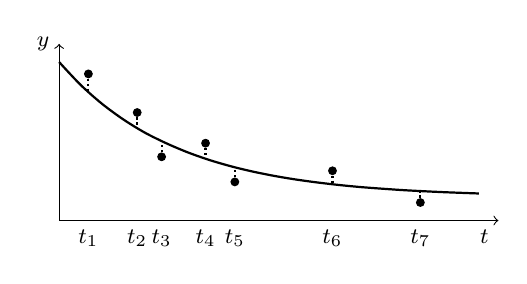
\begin{tikzpicture}[x=0.62cm,y=0.66cm]
        \draw[->] (0,0) -- (9.0,0) node[below left,font=\footnotesize] {$t$};
        \draw[->] (0,0) -- (0,3.4) node[left,font=\footnotesize] {$y$};
        \draw[thick] plot[smooth] coordinates {(0.00,3.050) (0.44,2.610) (0.88,2.245) (1.32,1.942) (1.76,1.689) (2.21,1.480) (2.65,1.306) (3.09,1.161) (3.53,1.041) (3.97,0.941) (4.41,0.858) (4.85,0.789) (5.29,0.732) (5.73,0.684) (6.17,0.644) (6.62,0.612) (7.06,0.584) (7.50,0.562) (7.94,0.543) (8.60,0.520)};
        \foreach \t/\y/\c in {0.60/2.821/2.471, 1.60/2.078/1.778, 2.10/1.226/1.526, 3.00/1.488/1.188, 3.60/0.743/1.023, 5.60/0.957/0.697, 7.40/0.346/0.566}{
          \draw[densely dotted,thick] (\t,\y) -- (\t,\c);
          \fill (\t,\y) circle (1.6pt);}
        \foreach \t/\l in {0.60/1,1.60/2,2.10/3,3.00/4,3.60/5,5.60/6,7.40/7}{\node[below,font=\footnotesize] at (\t,0) {$t_{\l}$};}
      \end{tikzpicture}\\
      {\small Figure 10.1 (redrawn)}
      \end{center}
    \end{column}
    \begin{column}{0.52\textwidth}
      Sum of the squared \emph{vertical} distances,
      \[ \tfrac12\sum_{j=1}^{m}\big[\phi(x;t_{j})-y_{j}\big]^{2}, \tag{10.7} \]
      which is (10.1) with
      \[ r_{j}(x)=\phi(x;t_{j})-y_{j} . \tag{10.8} \]
    \end{column}
  \end{columns}
\end{frame}

\begin{frame}{Why the sum of squares?}
  $\|r(x)\|_{\infty}$ or $\|r(x)\|_{1}$ \eqn{10.11} lead to smooth \emph{constrained} problems (Chapter 17);
  this chapter uses the $\ell_{2}$ form (10.1).

  \vspace{0.2em}
  \textbf{Statistical motivation.} Let $\epsilon_{j}=\phi(x;t_{j})-y_{j}$ be i.i.d.\ with density $g_{\sigma}$.
  The likelihood of the observations is
  \[ p(y;x,\sigma)=\prod_{j=1}^{m}g_{\sigma}(\epsilon_{j})=\prod_{j=1}^{m}g_{\sigma}(\phi(x;t_{j})-y_{j}) . \tag{10.12} \]
  For a normal distribution,
  $p(y;x,\sigma)=(2\pi\sigma^{2})^{-m/2}\exp\big(-\sum_{j}[\phi(x;t_{j})-y_{j}]^{2}/(2\sigma^{2})\big)$,
  so for fixed $\sigma$ \alert{the maximum likelihood estimate minimizes the sum of squares (10.7).}
\end{frame}

%=====================================================================
\section{\S10.2 Linear least squares}

\begin{frame}{Linear least-squares problems}
  If the model is linear in $x$, the residuals are linear: $r(x)=Jx-y$ with $J$, $y$ independent of $x$,
  \[ f(x)=\tfrac12\|Jx-y\|^{2},\qquad \gradf(x)=J^{T}(Jx-y),\qquad \hessf(x)=J^{T}J . \tag{10.13} \]
  $f$ is convex, so any $\xs$ with $\gradf(\xs)=0$ is a global minimizer (Theorem 2.5):
  \[ J^{T}J\xs=J^{T}y \qquad\text{(the \textbf{normal equations})}. \tag{10.14} \]
  Assume $m\ge n$ and $J$ of full column rank.

  \vspace{0.3em}
  \textbf{Algorithm 1: normal equations.} Form $J^{T}J$ and $J^{T}y$; Cholesky factorization
  $J^{T}J=\bar R^{T}\bar R$ \eqn{10.15}; two triangular substitutions.
  Drawback: $\kappa(J^{T}J)=\kappa(J)^{2}$; the factorization can break down when $J$ is ill conditioned.
\end{frame}

\begin{frame}{Algorithm 2: QR}
  The Euclidean norm is unchanged by orthogonal transformations:
  $\|Jx-y\|=\|Q^{T}(Jx-y)\|$ \eqn{10.16}. QR factorization with column pivoting,
  \[ J\Pi=Q\begin{bmatrix}R\\0\end{bmatrix}=\begin{bmatrix}Q_{1}&Q_{2}\end{bmatrix}\begin{bmatrix}R\\0\end{bmatrix}=Q_{1}R, \tag{10.17} \]
  $\Pi$ a permutation, $Q$ orthogonal $m\times m$, $R$ upper triangular $n\times n$. Then
  \[ \|Jx-y\|_{2}^{2}=\big\|R(\Pi^{T}x)-Q_{1}^{T}y\big\|_{2}^{2}+\big\|Q_{2}^{T}y\big\|_{2}^{2}, \tag{10.18} \]
  and $x$ affects only the first term: $\xs=\Pi R^{-1}Q_{1}^{T}y$ (solve $Rz=Q_{1}^{T}y$, permute).

  \vspace{0.3em}
  The error is proportional to the condition number of $J$, not its square. Usually reliable.
\end{frame}

\begin{frame}{Algorithm 3: SVD}
  \[ J=U\begin{bmatrix}S\\0\end{bmatrix}V^{T}=\begin{bmatrix}U_{1}&U_{2}\end{bmatrix}\begin{bmatrix}S\\0\end{bmatrix}V^{T}=U_{1}SV^{T}, \tag{10.19} \]
  $U$ ($m\times m$) and $V$ ($n\times n$) orthogonal, $S=\mathrm{diag}(\sigma_{1}\ge\cdots\ge\sigma_{n}>0)$.
  As in (10.18), $\|Jx-y\|^{2}=\|S(V^{T}x)-U_{1}^{T}y\|^{2}+\|U_{2}^{T}y\|^{2}$ \eqn{10.20}, hence
  \[ \xs=\sum_{i=1}^{n}\frac{u_{i}^{T}y}{\sigma_{i}}\,v_{i} . \tag{10.21} \]
  \begin{itemize}\setlength\itemsep{0.3em}
    \item \textbf{Sensitivity.} Small $\sigma_{i}$: $\xs$ is very sensitive to perturbations of $u_{i}^{T}y$.
    \item \textbf{Rank-deficient $J$} (some $\sigma_{i}=0$): every $\xs$ of the form (10.22), with arbitrary
      coefficients on those $v_{i}$, is a minimizer; zero coefficients give the smallest norm.
  \end{itemize}
\end{frame}

\begin{frame}{Choosing among the three; large problems}
  \begin{center}
  \small\setlength\tabcolsep{6pt}
  \begin{tabular}{lll}
    \toprule
    Method & Conditioning & When \\
    \midrule
    Normal equations & $\kappa(J)^{2}$ & $m\gg n$ or $J$ sparse: store $J^{T}J$, not $J$ \\
    QR & $\kappa(J)$ & usually reliable \\
    SVD & $\kappa(J)$ & most robust; sensitivity information; costliest \\
    \bottomrule
  \end{tabular}
  \end{center}

  \vspace{0.1em}
  \begin{itemize}\setlength\itemsep{0.3em}
    \item Ill-conditioned $J$: omitting the terms with small $\sigma_{i}$ from (10.21) gives an
      approximate solution that is less sensitive to perturbations.
    \item \textbf{Very large problems:} solve (10.14) by CG (Algorithm 5.2): one product with $J$ and
      one with $J^{T}$ per iteration, $J^{T}J$ never formed. LSQR (Paige and Saunders): same cost,
      better numerical properties.
  \end{itemize}
  \readbook{pp.~250--254.}
\end{frame}

%=====================================================================
\section{\S10.3 The Gauss--Newton method}

\begin{frame}{The Gauss--Newton method}
  Newton's method with line search would solve $\hessf(x_{k})p=-\gradf(x_{k})$.
  Gauss--Newton solves instead
  \[ J_{k}^{T}J_{k}\,p_{k}^{\GN}=-J_{k}^{T}r_{k}, \tag{10.23} \]
  that is, it uses the approximation
  \[ \hessf_{k}\approx J_{k}^{T}J_{k} . \tag{10.24} \]

  \begin{itemize}\setlength\itemsep{0.4em}
    \item \textbf{No second derivatives.} The individual residual Hessians $\nabla^{2}r_{j}$ in (10.5)
      are not needed. If $J_{k}$ is computed for the gradient anyway, (10.24) costs nothing more.
    \item \textbf{Often accurate.} When $J^{T}J$ dominates the second term of (10.5) near $\xs$
      (each $|r_{j}|\,\|\nabla^{2}r_{j}\|$ small), the convergence rate is similar to Newton's.
  \end{itemize}
\end{frame}

\begin{frame}{Two more advantages}
  \textbf{Descent.} If $J_{k}$ has full rank and $\gradf_{k}\ne 0$, then by (10.4) and (10.23)
  \[
    (p_{k}^{\GN})^{T}\gradf_{k}=(p_{k}^{\GN})^{T}J_{k}^{T}r_{k}=-(p_{k}^{\GN})^{T}J_{k}^{T}J_{k}p_{k}^{\GN}=-\|J_{k}p_{k}^{\GN}\|^{2}\le 0 ,
    \tag{10.25}
  \]
  with equality only if $J_{k}p_{k}^{\GN}=0$, which means $J_{k}^{T}r_{k}=\gradf_{k}=0$.
  So $p_{k}^{\GN}$ is a descent direction, suitable for a line search (Armijo or Wolfe, (3.4), (3.6)).

  \vspace{0.4em}
  \textbf{A linear least-squares subproblem.} (10.23) are the normal equations of
  \[ \min_{p}\ \tfrac12\|J_{k}p+r_{k}\|^{2} . \tag{10.26} \]
  So $p_{k}^{\GN}$ can be computed by QR or SVD of $J_{k}$, or by CG, \alert{without forming $J_{k}^{T}J_{k}$}.
  ($m$ large, $n$ small: do not store $J$; accumulate $J^{T}J$ and $J^{T}r$ residual by residual \eqn{10.27}.)
\end{frame}

\begin{frame}{Gauss--Newton as a linear model of the residuals}
  Subproblem (10.26) comes from the linear model $r(x_{k}+p)\approx r_{k}+J_{k}p$ substituted
  into $\tfrac12\|\cdot\|^{2}$:
  \[ f(x_{k}+p)=\tfrac12\|r(x_{k}+p)\|^{2}\approx\tfrac12\|J_{k}p+r_{k}\|^{2} , \]
  and $p_{k}^{\GN}$ is the minimizer of this approximation.

  \vspace{0.6em}
  \begin{block}{Comparison with Chapter 6 \notinbook}
    Both methods replace $\hessf_{k}$ by a matrix $B_{k}$ built from first derivatives.
    Quasi-Newton builds $B_{k}$ from the history of gradient differences and must enforce
    $s_{k}^{T}y_{k}>0$. Gauss--Newton takes $B_{k}=J_{k}^{T}J_{k}$ from the current Jacobian;
    it is positive semidefinite by construction.
  \end{block}
\end{frame}

\begin{frame}{Theorem 10.1: global convergence of Gauss--Newton}
  Uniform full-rank condition \eqn{10.28}: $\|J(x)z\|\ge\gamma\|z\|$ on $\Ncal\supset\Lcal=\{x\,|\,f(x)\le f(x_{0})\}$.

  \begin{block}{Theorem 10.1}
    Suppose each residual function $r_{j}$ is Lipschitz continuously differentiable in a
    neighborhood $\Ncal$ of the bounded level set (10.29), and that the Jacobians $J(x)$ satisfy the
    uniform full-rank condition (10.28) on $\Ncal$. Then if the iterates $x_{k}$ are generated by the
    Gauss--Newton method with step lengths $\alpha_{k}$ that satisfy (3.6), we have
    \[ \lim_{k\to\infty}J_{k}^{T}r_{k}=0 . \]
  \end{block}

  Zoutendijk (Theorem 3.2) with $\cos\theta_{k}\ge\gamma^{2}/\bar\beta^{2}>0$ by (10.28). \readbook{proof, p.~256.}
\end{frame}

\begin{frame}{Local convergence of Gauss--Newton}
  Let $H(x)$ denote the second-order term $\sum_{j}r_{j}(x)\nabla^{2}r_{j}(x)$ of (10.5), and
  write $J^{T}J(x)$ for $J(x)^{T}J(x)$. For a unit step, an argument like (3.31)--(3.33) gives
  \[
    \|x_{k}+p_{k}^{\GN}-\xs\|\ \approx\ \big\|[J^{T}J(\xs)]^{-1}H(\xs)\big\|\,\|x_{k}-\xs\|+O(\|x_{k}-\xs\|^{2}) .
    \tag{10.30}
  \]
  \begin{itemize}\setlength\itemsep{0.5em}
    \item If $\|[J^{T}J(\xs)]^{-1}H(\xs)\|\ll 1$, a unit Gauss--Newton step moves much closer to $\xs$:
      rapid local convergence.
    \item If $H(\xs)=0$ (zero residual): quadratic convergence.
    \item Otherwise the rate is linear, with factor $\|[J^{T}J(\xs)]^{-1}H(\xs)\|$.
  \end{itemize}
  \readbook{p.~257.}
\end{frame}

\begin{frame}{Rank-deficient Jacobians; inexact Gauss--Newton}
  \begin{itemize}\setlength\itemsep{0.6em}
    \item If $J_{k}$ is rank-deficient, (10.23) is singular but still solvable, because it is
      equivalent to (10.26); the solutions have the form (10.22).
    \item Then $\cos\theta_{k}$ is no longer bounded away from zero, and a result like Theorem 10.1
      cannot be proved. (Levenberg--Marquardt removes this weakness.)
    \item \textbf{Inexact Gauss--Newton.} When $n$ and $m$ are large and $J$ is sparse, factoring $J_{k}$
      or $J_{k}^{T}J_{k}$ at every iteration is expensive. Use the inexact Newton methods of
      Chapter 7 with $J_{k}^{T}J_{k}$ in place of $\hessf_{k}$; its positive semidefiniteness
      simplifies them.
  \end{itemize}
\end{frame}

%=====================================================================
\section{\S10.3 The Levenberg--Marquardt method}

\begin{frame}{The Levenberg--Marquardt method}
  Approximation (10.24) inside a \alert{trust region}; rank-deficient $J$ is no longer a difficulty:
  \[ \min_{p}\ \tfrac12\|J_{k}p+r_{k}\|^{2},\qquad\text{subject to }\|p\|\le\Delta_{k}, \tag{10.31} \]
  that is, the model function of (4.3) is
  \[ m_{k}(p)=\tfrac12\|r_{k}\|^{2}+p^{T}J_{k}^{T}r_{k}+\tfrac12p^{T}J_{k}^{T}J_{k}p . \tag{10.32} \]
  Drop the index $k$. If $\|p^{\GN}\|<\Delta$, then $p^{\GN}$ solves (10.31). Otherwise there is
  $\lambda>0$ such that the solution $p=p^{\LM}$ satisfies $\|p\|=\Delta$ and
  \[ (J^{T}J+\lambda I)\,p=-J^{T}r . \tag{10.33} \]
\end{frame}

\begin{frame}{Lemma 10.2}
  \begin{block}{Lemma 10.2}
    The vector $p^{\LM}$ is a solution of the trust-region subproblem
    \[ \min_{p}\ \|Jp+r\|^{2},\qquad\text{subject to }\|p\|\le\Delta, \]
    if and only if $p^{\LM}$ is feasible and there is a scalar $\lambda\ge 0$ such that
    \begin{align}
      (J^{T}J+\lambda I)\,p^{\LM}&=-J^{T}r, \tag{10.34a}\\
      \lambda(\Delta-\|p^{\LM}\|)&=0 . \tag{10.34b}
    \end{align}
  \end{block}

  \vspace{0.2em}
  Theorem 4.1 applied; (4.8c) holds since $J^{T}J\succeq 0$, $\lambda\ge 0$. \readbook{proof, p.~259.}
\end{frame}

\begin{frame}{Computing the Levenberg--Marquardt step}
  (10.33) are the normal equations of a linear least-squares problem,
  \[ \min_{p}\ \tfrac12\Big\|\begin{bmatrix}J\\ \sqrt{\lambda}\,I\end{bmatrix}p+\begin{bmatrix}r\\0\end{bmatrix}\Big\|^{2}, \tag{10.35} \]
  so the step is computed without forming $J^{T}J$. Find $\lambda$ from $\Delta$ by rootfinding (Ch.~4).

  \vspace{0.2em}
  \textbf{QR for several $\lambda$.} Householder QR of $J$ once \eqn{10.37}; then, for each $\lambda$,
  $n(n+1)/2$ Givens rotations:
  \[ \begin{bmatrix}R_{\lambda}\\0\end{bmatrix}=Q_{\lambda}^{T}\begin{bmatrix}J\\ \sqrt{\lambda}\,I\end{bmatrix},\qquad R_{\lambda}^{T}R_{\lambda}=J^{T}J+\lambda I . \tag{10.36} \]
  Cost: $O(mn^{2})$ once, then $O(n^{3})$ per value of $\lambda$. \readbook{pp.~259--260.}
\end{frame}

\begin{frame}{Scaling; large sparse problems}
  \begin{itemize}\setlength\itemsep{0.5em}
    \item Least-squares problems are often poorly scaled: some variables of size $10^{4}$,
      others $10^{-6}$. Use an \textbf{ellipsoidal} trust region with a diagonal $D_{k}$:
  \end{itemize}
  \[ \min_{p}\ \tfrac12\|J_{k}p+r_{k}\|^{2},\qquad\text{subject to }\|D_{k}p\|\le\Delta_{k}, \tag{10.39} \]
  \[ \big(J_{k}^{T}J_{k}+\lambda D_{k}^{2}\big)\,p_{k}^{\LM}=-J_{k}^{T}r_{k} . \tag{10.40} \]
  \begin{itemize}\setlength\itemsep{0.5em}
    \item[] Seber and Wild: match the diagonal of $D_{k}^{2}$ to that of $J_{k}^{T}J_{k}$, which makes the
      algorithm invariant under diagonal scaling of $x$ (cf.\ Section 4.5).
    \item \textbf{Large sparse $J$:} solve (10.31) or (10.39) approximately by CG--Steihaug
      (Algorithm 7.2) with $J_{k}^{T}J_{k}$. No negative curvature can arise, and only products
      with $J_{k}$ and $J_{k}^{T}$ are needed. \readbook{pp.~260--261.}
  \end{itemize}
\end{frame}

\begin{frame}{Theorem 10.3: global convergence of Levenberg--Marquardt}
  \begin{block}{Theorem 10.3}\small
    Let $\eta\in(0,\tfrac14)$ in Algorithm 4.1 of Chapter 4, and suppose that the level set $\Lcal$ defined in
    (10.29) is bounded and that the residual functions $r_{j}(\cdot)$, $j=1,2,\dots,m$ are Lipschitz
    continuously differentiable in a neighborhood $\Ncal$ of $\Lcal$. Assume that for each $k$, the
    approximate solution $p_{k}$ of (10.31) satisfies the inequality
    \[ m_{k}(0)-m_{k}(p_{k})\ge c_{1}\|J_{k}^{T}r_{k}\|\min\Big(\Delta_{k},\frac{\|J_{k}^{T}r_{k}\|}{\|J_{k}^{T}J_{k}\|}\Big), \tag{10.42} \]
    for some constant $c_{1}>0$, and in addition $\|p_{k}\|\le\gamma\Delta_{k}$ for some constant $\gamma\ge 1$.
    We then have that $\lim_{k\to\infty}\gradf_{k}=\lim_{k\to\infty}J_{k}^{T}r_{k}=0$.
  \end{block}

  Theorem 4.6 applied; (10.42) is the Cauchy-point decrease. \readbook{proof, p.~262.}
\end{frame}

\begin{frame}{Local behavior; large-residual problems}
  Near a solution $\xs$ where $J^{T}J$ dominates, the trust region becomes inactive and the
  algorithm takes Gauss--Newton steps: the local rate is again (10.30).

  \vspace{0.4em}
  \begin{alertblock}{Large-residual problems}
    If the second-order part of $\hessf$ is too large to ignore, the model (10.31) is inadequate.
    Gauss--Newton and Levenberg--Marquardt then converge only \alert{linearly}, slower than
    Newton or quasi-Newton methods.
  \end{alertblock}

  \begin{itemize}\setlength\itemsep{0.3em}
    \item If the $\nabla^{2}r_{j}$ are easy to compute: Newton's method with a trust region or line search.
      Otherwise quasi-Newton (superlinear). But both may be worse than Gauss--Newton in the
      early iterations.
    \item Large residuals at the solution often mean the model is inadequate or the data are wrong.
  \end{itemize}
\end{frame}

\begin{frame}{Hybrid methods}
  We rarely know in advance whether the residuals at the solution will be small or large.
  Hybrid algorithms behave like Gauss--Newton when they are small, and switch to Newton or
  quasi-Newton steps otherwise.

  \begin{itemize}\setlength\itemsep{0.5em}
    \item \textbf{Fletcher and Xu.} If the Gauss--Newton step reduces $f$ by a fixed factor (say 5),
      take it and set $B_{k}\la J_{k}^{T}J_{k}$; otherwise take a line-search step along $-B_{k}^{-1}\gradf_{k}$.
      Then apply a BFGS-like update to $B_{k}$. Zero residual: eventually Gauss--Newton
      (quadratic). Nonzero residual: eventually BFGS (superlinear).
    \item \textbf{Dennis, Gay, and Welsch (NL2SOL).} Keep $J_{k}^{T}J_{k}$; approximate the rest:
  \end{itemize}
  \[ B_{k}=J_{k}^{T}J_{k}+S_{k},\qquad S_{k}\approx\sum_{j=1}^{m}r_{j}(x_{k})\nabla^{2}r_{j}(x_{k}) . \]
\end{frame}

\begin{frame}{The Dennis--Gay--Welsch update}
  Each $(B_{j})_{k+1}\approx\nabla^{2}r_{j}$ should mimic the change of $\nabla r_{j}$ over the step;
  weighted by $r_{j}(x_{k+1})$ and summed, a \textbf{secant equation} for $S_{k+1}$:
  \[ S_{k+1}(x_{k+1}-x_{k})=J_{k+1}^{T}r_{k+1}-J_{k}^{T}r_{k+1} . \]
  With symmetry and closeness to $S_{k}$ (as in Chapter 6),
  \[
    S_{k+1}=S_{k}+\frac{(y^{\sharp}-S_{k}s)y^{T}+y(y^{\sharp}-S_{k}s)^{T}}{y^{T}s}
    -\frac{(y^{\sharp}-S_{k}s)^{T}s}{(y^{T}s)^{2}}\,yy^{T},
    \tag{10.43}
  \]
  \[ s=x_{k+1}-x_{k},\qquad y=J_{k+1}^{T}r_{k+1}-J_{k}^{T}r_{k},\qquad y^{\sharp}=J_{k+1}^{T}r_{k+1}-J_{k}^{T}r_{k+1} . \]
  A variant of DFP (identical if $y^{\sharp}=y$). $S_{k}$ is scaled down before each update, so it can
  vanish on zero-residual problems. \readbook{pp.~263--265.}
\end{frame}

%=====================================================================
\section{\S10.4 Orthogonal distance regression}

\begin{frame}{Orthogonal distance regression}
  Errors in the $t_{j}$ as well (\emph{errors-in-variables}): perturbations $\delta_{j}$,
  \[ y_{j}=\phi(x;t_{j}+\delta_{j})+\epsilon_{j},\qquad j=1,2,\dots,m, \tag{10.44} \]
  \[ \min_{x,\delta_{j},\epsilon_{j}}\ \tfrac12\sum_{j=1}^{m}w_{j}^{2}\epsilon_{j}^{2}+d_{j}^{2}\delta_{j}^{2},\qquad\text{subject to (10.44)}. \tag{10.45} \]
  \begin{columns}[T,onlytextwidth]
    \begin{column}{0.44\textwidth}
      \begin{center}
      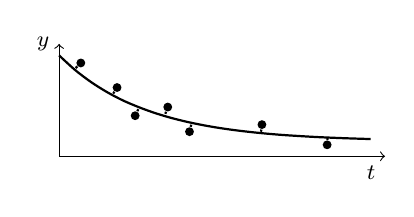
\begin{tikzpicture}[x=0.46cm,y=0.42cm]
        \draw[->] (0,0) -- (9.0,0) node[below left,font=\footnotesize] {$t$};
        \draw[->] (0,0) -- (0,3.4) node[left,font=\footnotesize] {$y$};
        \draw[thick] plot[smooth] coordinates {(0.00,3.050) (0.44,2.610) (0.88,2.245) (1.32,1.942) (1.76,1.689) (2.21,1.480) (2.65,1.306) (3.09,1.161) (3.53,1.041) (3.97,0.941) (4.41,0.858) (4.85,0.789) (5.29,0.732) (5.73,0.684) (6.17,0.644) (6.62,0.612) (7.06,0.584) (7.50,0.562) (7.94,0.543) (8.60,0.520)};
        \foreach \t/\y/\u/\v in {0.60/2.821/0.42/2.627, 1.60/2.078/1.47/1.853, 2.10/1.226/2.21/1.478, 3.00/1.488/2.91/1.215, 3.60/0.743/3.66/1.008, 5.60/0.957/5.57/0.700, 7.40/0.346/7.41/0.566}{
          \draw[densely dotted,thick] (\t,\y) -- (\u,\v);
          \fill (\t,\y) circle (1.6pt);}
      \end{tikzpicture}
      \end{center}
    \end{column}
    \begin{column}{0.54\textwidth}
      \small Figure 10.2 (redrawn). With $w_{j}=d_{j}$, each term of (10.45) is the shortest distance
      from $(t_{j},y_{j})$ to the curve; the shortest path meets the curve orthogonally.
      Linear case: \emph{total least squares}.
    \end{column}
  \end{columns}
\end{frame}

\begin{frame}{ODR as a least-squares problem with structure}
  Eliminate $\epsilon_{j}$ by (10.44): unconstrained, $2m$ residuals, $n+m$ unknowns,
  \[
    \min_{x,\delta}\ F(x,\delta)=\tfrac12\sum_{j=1}^{m}w_{j}^{2}[y_{j}-\phi(x;t_{j}+\delta_{j})]^{2}+d_{j}^{2}\delta_{j}^{2}
    =\tfrac12\sum_{j=1}^{2m}r_{j}^{2}(x,\delta) .
    \tag{10.46}
  \]
  Since $\partial r_{j}/\partial\delta_{i}=0$ for $i\ne j$ and $\partial r_{m+j}/\partial x_{i}=0$,
  \[ J(x,\delta)=\begin{bmatrix}\hat J&V\\0&D\end{bmatrix}, \tag{10.48} \]
  $V$, $D$ diagonal; $\hat J$ the $m\times n$ Jacobian of $w_{j}\phi(t_{j}+\delta_{j};x)$ in $x$. In (10.33)
  partitioned as (10.49), the block $V^{2}+D^{2}+\lambda I$ is diagonal: eliminate $p_{\delta}$, solve
  an $n\times n$ system for $p_{x}$. \readbook{pp.~265--267.}
\end{frame}

%=====================================================================
\section{Chapter 10: summary}

\begin{frame}{Perspectives and software}
  \begin{itemize}\setlength\itemsep{0.45em}
    \item The original Levenberg--Marquardt algorithm adjusted $\lambda$ in (10.33) directly, increasing
      or decreasing it by a factor according to whether the previous step decreased $f$. The
      connection with trust regions was established by Mor\'e.
    \item \textbf{Inexact Levenberg--Marquardt} (Wright and Holt): steps $\bar p_{k}$ with
  \end{itemize}
  \[ \big\|(J_{k}^{T}J_{k}+\lambda_{k}I)\bar p_{k}+J_{k}^{T}r_{k}\big\|\le\eta_{k}\|J_{k}^{T}r_{k}\|,\qquad\eta_{k}\in[0,\eta], \]
  \begin{itemize}\setlength\itemsep{0.45em}
    \item[] a forcing sequence as in (7.3). Implemented with LSQR, which gives approximate
      solutions of (10.35) for several $\lambda_{k}$ at once.
    \item Software: IMSL, HSL, NAG, SAS; DFNLP, MINPACK, NL2SOL, NLSSOL; LANCELOT, KNITRO, SNOPT
      (large scale); ORDPACK (ODR). All accept Jacobians or compute them by finite differencing.
  \end{itemize}
\end{frame}

\begin{frame}{Two uses of this chapter \notinbook}
  \begin{block}{Power system state estimation}
    Weighted least squares $\min_{x}\tfrac12(z-h(x))^{T}W(z-h(x))$: measurements $z$, power-flow
    equations $h$. The standard algorithm is Gauss--Newton with weights: the ``gain matrix''
    $H^{T}WH$ is $J^{T}J$ of (10.23), observability is the rank condition (10.28), and bad-data
    detection is residual analysis.
  \end{block}

  \begin{block}{Machine learning}
    With a squared-error loss, training is (10.1) and $J^{T}J$ is the Gauss--Newton matrix; for
    other losses the same construction is called generalized Gauss--Newton. The Shampoo
    preconditioner can be viewed as a Kronecker approximation of the Gauss--Newton part of the
    Hessian (Morwani et al., ICLR 2025): see the November presentations.
  \end{block}
\end{frame}

\begin{frame}{Chapter 10 in one table}
  \begin{center}
  \small\setlength\tabcolsep{5pt}
  \begin{tabular}{llll}
    \toprule
    Method & Hessian model & Globalization & Local rate \\
    \midrule
    Gauss--Newton & $J^{T}J$ & line search & (10.30); quadratic if $H(\xs)=0$ \\
    Levenberg--Marquardt & $J^{T}J$ & trust region & same as Gauss--Newton \\
    Fletcher--Xu hybrid & $J^{T}J$ or BFGS & line search & quadratic or superlinear \\
    Dennis--Gay--Welsch & $J^{T}J+S_{k}$ & trust region & superlinear \\
    Newton & (10.5) & either & quadratic \\
    \bottomrule
  \end{tabular}
  \end{center}

  \vspace{0.4em}
  \begin{itemize}\setlength\itemsep{0.4em}
    \item Small residuals: Gauss--Newton or Levenberg--Marquardt; the rate is nearly quadratic.
    \item Large residuals: their rate is linear; use Newton, quasi-Newton, or a hybrid.
    \item Rank-deficient or ill-conditioned $J$: Levenberg--Marquardt, not Gauss--Newton.
  \end{itemize}
\end{frame}

\begin{frame}{Three results to carry forward}
  \begin{enumerate}\setlength\itemsep{0.7em}
    \item \textbf{$J^{T}J$ is the part of the Hessian that comes with the gradient.} Its quality as an
      approximation is governed by the residuals, (10.5) and (10.30): small residuals, fast
      convergence; large residuals, linear convergence.
    \item \textbf{Gauss--Newton is Newton's method with $B_{k}=J_{k}^{T}J_{k}$; Levenberg--Marquardt is
      the same model in a trust region.} $(J^{T}J+\lambda I)p=-J^{T}r$ is the trust-region step
      (Lemma 10.2), and the global theory is Chapter 3 and Chapter 4 applied.
    \item \textbf{Never form $J^{T}J$ unless $m\gg n$.} The step solves a linear least-squares problem,
      (10.26) or (10.35), by QR, SVD or CG/LSQR on $J$ itself.
  \end{enumerate}

  \vspace{0.6em}
  Proved in the book: Theorem 10.1, Lemma 10.2, Theorem 10.3. Derivation only: (10.30).
\end{frame}

\begin{frame}{Homework {\normalfont\small(problems 4--5 are not in the book)}}
  \begin{enumerate}\setlength\itemsep{0.45em}
    \item Exercise 10.1(a): $J$ ($m\times n$, $m\ge n$) has full column rank if and only if $J^{T}J$ is nonsingular.
    \item Exercise 10.2: show that the function $f(x)$ in (10.13) is convex.
    \item Exercise 10.3(a): if $Q$ is orthogonal, then $\|Qx\|=\|x\|$ for any vector $x$.
    \item By hand. $n=1$, $m=2$, $r_{1}(x)=x-2$, $r_{2}(x)=x^{2}-1$, $x_{0}=0$. Compute the
      Gauss--Newton step (10.23), the Levenberg--Marquardt step (10.33) with $\lambda=1$, and the
      Newton step. Which of the three are descent directions, and why?
    \item Implement Gauss--Newton with your Chapter 3 line search for the model (10.6):
      generate data from $x=(1,0,0,2,1)$ at $t_{j}=1,\dots,7$ with small Gaussian noise, and fit
      from $x_{0}=(0,0,0,1,0.5)$. Compare the iterates with \texttt{scipy.optimize.least\_squares}.
  \end{enumerate}
\end{frame}

\end{document}
